\documentclass{rpt}

\begin{document}
\subsubsection*{Questions on \textit{mfs}}

\begin{enumerate}
\item Is \textit{mfs} a state-of-the-art method for logic synthesis with EXDCs?
\item Is \textit{mfs} only designed for FPGAs? Does it also work for ASICs?
\end{enumerate}

\subsubsection*{Questions on my research with \textit{mfs}}

The idea is to generate approximate circuits by approximating its EXDCs with logic simulation.
I start from the \textit{mfs} method in the paper \textit{Scalable Don't-Care-Based Logic Optimization and Resynthesis}.
The {\bf only} change is the structure of miter in Figure~\ref{fig:ori} (the Figure 4.2.1 in the \textit{mfs} paper).

\begin{figure}[!htbp]
\centering
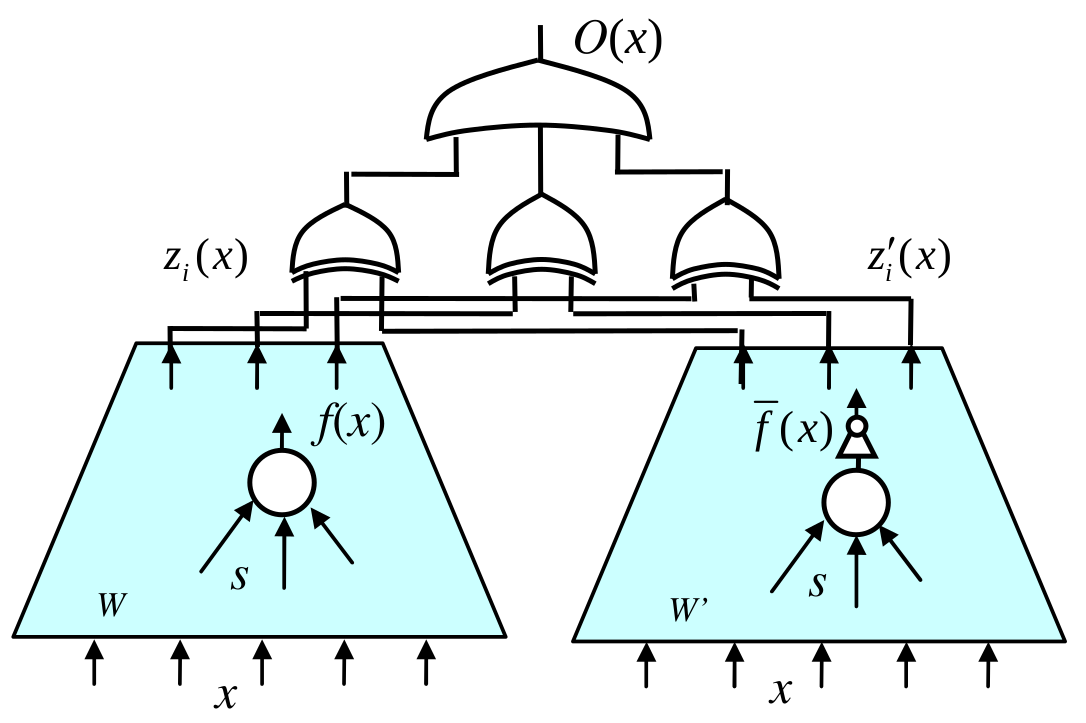
\includegraphics[scale = 0.2]{./sat.png}
\caption{Original miter for care set computation}\label{fig:ori}
\end{figure}

Instead of constructing such a miter in Figure~\ref{fig:ori} to represent the care set,
I simulate the circuit for $N$ rounds and generate a set of patterns for window inputs $\mathbf{x}$.
Those patterns are treated as the {\bf approximate care set} and used to synthesize the approximate circuit.

For example, the window inputs are $A$, $B$ and $C$, and three rounds simulation patterns for $ABC$ are 010, 111, 101.
Then I use $O(x) = \overline AB \overline C + ABC + A \overline B C$ to represent the approximate care set.

\begin{enumerate}
\item Is the modification on \textit{mfs} reasonable to generate approximate designs?
\item I have an interesting observation on \textit{c880} with my idea:

\begin{enumerate}[(a)]
\item
In most cases, for some values of $N$ within a continuous interval,
the final approximate circuit does not change.
For example,
I increase $N$ from 192 to 256, the results are same.

\item
But the error rate of the approximate circuit might change dramatically due to the addition of one simulation frame.
For example, when $N$ change from 256 to 257 (the first 256 inputs patterns for simulation are same), the error rate of the final circuit changes greatly (from 0.2\% to 5\%).
\end{enumerate}

Is the observation caused by the property of \textit{mfs}?
\end{enumerate}

\end{document}
